\section{Corrections to the Hydrogen Atom Continued}
\subsection{Review of Last Lecture}
We started to discuss a real hydrogen atom which exists in nature. We did estimates for the so-called ``fine structure'' of the hydrogen atom. We call:
\begin{equation}
    \alpha = \frac{e^2}{\hbar c}
\end{equation}
the fine structure coupling constant. The relativistic and spin-orbit corrections were of order $\alpha^2$. The hyperfine structure (which we will discuss in a few lectures) was of order $\alpha^210^{-3}$. There are also a few other effects; for example the Zeeman splitting from the Earth's magnetic field, and the Lamb shift which can be calculated from QFT (virtual pair production\ldots) which is given by:
\begin{equation}
    \Delta E = \frac{\alpha^3}{6\pi}\si{Ry}\ln\left(\frac{1}{\pi\alpha}\right)
\end{equation}
Note that this has been measured, and this was computed by Feynman to high precision; leading to the birth of QFT! 

\subsection{Relativistic Correction - Computation}
We calculated the relativistic correction last class:
\begin{equation}
    \Delta E_{rel}^{(1)} = -\frac{1}{2mc^2}\left[E_n^2 + 2E_n\avg{\frac{e^2}{r}} + \avg{\frac{e^4}{r^2}}\right]
\end{equation}
where $E_n = \si{Ry}\left(-\frac{1}{2n^2}\right)$. The logic behind this was $\ket{n, l, m}$ are eigenstates of the unperturbed Hamiltonian:
\begin{equation}
    H^{0} = \frac{p^2}{2m} + V(r)
\end{equation}
We could then express $p^4$ (the relativistic correction) in terms of $H$ and hence obtain an expression in terms of eigenenergies. The remaining step is to compute the expectation values.

\subsubsection{The Feynman-Hellman Theorem}
Let:
\begin{equation}
    E_n(\lambda) = \bra{n}H(\lambda)\ket{n}.
\end{equation}
Then:
\begin{equation}
    \dpd{E_n}{\lambda} = \bra{n}\dpd{H}{n}\ket{n}
\end{equation}

\textit{Proof.} We compute using the product rule:
\begin{equation}\label{eq-productruleFeynman}
    \begin{split}
        \dpd{E_n}{\lambda} = \left(\dpd{}{\lambda}\bra{n}\right)H(\lambda)\ket{n(\lambda)} + \bra{n}\dpd{H}{n}\ket{n} + \bra{n}H\ket{\dpd{n}{\lambda}}
    \end{split}
\end{equation}
Now, since $\braket{n}{n} = 1$, it follows that:
\begin{equation}
    \dpd{}{\lambda}\braket{n}{n} = 0.
\end{equation}
And therefore:
\begin{equation}
    \dpd{}{\lambda}\braket{n}{n} = \left(\dpd{}{\lambda}\bra{n}\right)\ket{n} + \braket{n}{\dpd{n}{\lambda}} = 0
\end{equation}
and so the first/last terms in Eq. \eqref{eq-productruleFeynman} vanish, and we are left with the result. \qed

\subsubsection{Applying the Feynman-Hellman Theorem}
We have the known standard integral:
\begin{equation}
    \int_{-\infty}^\infty e^{-ax^2}dx = \sqrt{\frac{\pi}{a}}
\end{equation}
which can be computed by the trick of going into polar coordinates. We can then obtain the solution for whole families of integrals, e.g.:
\begin{equation}
    \int_{-\infty}^\infty x^2e^{-ax^2}dx = \dpd{}{a}\sqrt{\frac{\pi}{a}}
\end{equation}

\subsubsection{Applying the Feynman-Hellman Theorem for Relativistic Corrections}
We have:
\begin{equation}
    H^{(0)} = -\frac{\hbar^2}{2mr^2}\dpd{}{r}\left(r^2\dpd{}{r}\right) + \frac{\hbar^2l(l+1)}{2mr^2} - \frac{e^2}{r}
\end{equation}
Now we observe:
\begin{equation}
    \dpd{E_n}{(e^2)} = -\frac{2me^2}{2\hbar^2}\frac{1}{n^2} = \avg{-\frac{1}{r}}
\end{equation}
How did we know to pick this? We have to be a bit smart and choose to differentiate with respect to the variable that gives us the result we want. Next, we will want to differente w.r.t $l$. Recall however that $n$ depends on $l$:
\begin{equation}
    n = n_r + l + 1
\end{equation}
where $n_r$ is the radial quantum number and $l$ is the angular (and $n$ is the composite, principle quantum number). When we differentiate w.r.t. $l$, we get:
\begin{equation}
    \dpd{H^{(0)}}{l} = \frac{(2l+1)\hbar^2}{2mr^2}
\end{equation}
\begin{equation}
    \dpd{E_n}{l} = \frac{me^4}{\hbar^2(n_r + l + 1)^3}
\end{equation}
Since the expectation value of the first term must be equal to the second by the theorem, we can solve for what $\avg{\frac{1}{r^2}}$ should be. If we put everything in, we get:
\begin{equation}
    \Delta E_{rel}^{(1)} = -\frac{1}{2mc^2}\left[E_n^2 + 2E_n\avg{\frac{e^2}{r}} + \avg{\frac{e^4}{r^2}}\right] = \left(\frac{me^4}{\hbar^2}\right)\frac{\alpha^2}{(2n^2)^2}\left(-\frac{1}{2}\right)\left(\frac{4n}{l+\frac{1}{2}} - 3\right)
\end{equation}

So we get the $\propto\alpha^2$ from our order of magnitude calculation! This is not at all surprising, because all the terms we add together are of the same order, and:
\begin{equation}
    \frac{1}{mc^2}\left(\frac{me^4}{\hbar^2}\right)^2 = \left(\frac{me^4}{\hbar^2}\right)\left(\frac{me^4}{\hbar^2mc^2}\right) = \alpha^2
\end{equation}

Some important notes: we see a dependence on $l$ in our relativistic correction, and of course it should appear in all of our computations. 2s and 2p orbitals would have different corrections. Second remark; why can we use PT without degeneracy when we have huge degeneracy of $g = 2n^2$? Because our perturbing Hamiltonian commutes with our classification scheme.

\subsection{Spin-Orbit Correction - Calculation}
We start with the Hamiltonian:
\begin{equation}
    H_{SO} = -\gv{mu} \cdot \v{B}
\end{equation}
where $\v{B}$ is a classical (dipole - from multipole expansion) field:
\begin{equation}
    \v{B} = \frac{\abs{e}}{c}\frac{\v{v} \times \v{r}}{r^3} = \frac{\abs{e}}{\hbar c}\frac{\v{L}}{r^3}
\end{equation}
and we have:
\begin{equation}
    \mu = -\frac{\abs{e}\hbar}{2mc}(2\v{S})
\end{equation}
therefore:
\begin{equation}
    H_{SO} = \frac{e^2\hbar^2}{2m^2c^2}\frac{\v{S} \cdot \v{L}}{r^3}.
\end{equation}
We now define $\v{J} = \v{L} + \v{S}$ as usual, and observing that:
\begin{equation}
    [H_{SO}, \v{J}_i] = 0
\end{equation}
we conclude that we can use the $\ket{n, l, s=1/2, j, j_z}$ basis/classification in our perturbation theory, and we can use the non-degenerate PT technique as $\v{J}$ commutes with the Hamiltonian. We are interested in:
\begin{equation}
    \bra{n,l,s=1/2, j, j_z}\v{L} \cdot \v{S}\ket{n,l,s=1/2, j, j_z}
\end{equation}
But since:
\begin{equation}
    \v{L}\cdot \v{S} = \frac{1}{2}\left(\v{J}^2 - \v{S}^2 - \v{L}^2\right)
\end{equation}
we then have:
\begin{equation}
    \bra{n,l,s=1/2, j, j_z}\v{L} \cdot \v{S}\ket{n,l,s=1/2, j, j_z} = \frac{1}{2}\left(j(j+1) - \frac{3}{4} - l(l+1)\right).
\end{equation}

We still need to compute $\avg{\frac{1}{r^3}}$. We can use Kramer's Relation (whose proof comes down to integration by parts):
\begin{equation}
    \avg{\frac{1}{r^3}} = \frac{1}{a_B^3}\frac{1}{n^3(l + \frac{1}{2})l(l+1)}
\end{equation}
From this we can obtain the full solution:

\begin{equation}
    \avg{H^{(1)}} = \frac{e^2\hbar^2}{2m^2c^2}\frac{1}{a_B^3}\frac{j(j+1) - \frac{3}{4} - l(l+1)}{2n^3(l + \frac{1}{2})l(l+1)}
\end{equation}
But let's look at the constant prefactor here:
\begin{equation}
    \frac{e^2\hbar^2}{2m^2c^2}\left(\frac{me^2}{\hbar^2}\right)^3 = \frac{me^4}{2\hbar^2}\left(\frac{e^2}{\hbar c}\right)^2 = \si{Ry}\alpha^2
\end{equation}
so again we see that our order of magnitude prediction of $\propto \alpha^2$ checks out!

\subsection{Combining the Corrections}
In sum, the fine structure corrections to the hydrogen atom are given by:
\begin{equation}\label{eq-finestructurecorrection}
    \Delta E_{SO}^{(1)} + \Delta E_{rel}^{(1)} = -\frac{me^4}{\hbar^2}\frac{\alpha^2}{2n}\left[\frac{n}{j+\frac{1}{2}} - \frac{3}{4}\right]
\end{equation}
If we plot the energy levels with the fine structure corrections, we obtain Fig. \ref{fig-finestructuresplit}.

\begin{figure}[htbp]
    \centering
    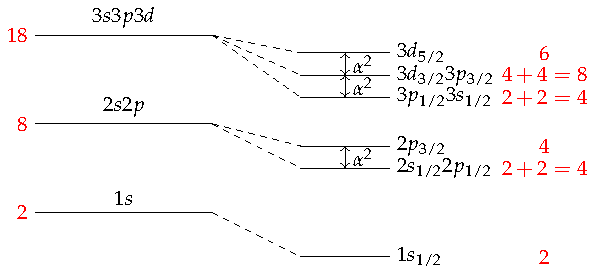
\includegraphics[]{Images/fig-finestructuresplit.pdf}

    \caption{The energy levels of the hydrogen atom split due to the relativistic and spin-orbit corrections. The figure is not drawn to scale. The old classification with degeneracy counting is on the left. The new classification with appropriate energy splitting and degeneracy counting is on the right.}
    \label{fig-finestructuresplit}
\end{figure}

We notice something very intriguing about the energy correction in Eq. \eqref{eq-finestructurecorrection}; the net result does \emph{not} have any dependence on $l$ (only on $j$). It is extremely nontrivial. For any potential in the world, we would have an $l$ dependence; but for this \emph{very} special (unique! - for further reading see the Runge Lentz vector and its connection to $1/r^2$ potentials) case, we have this $l$-indepenent structure. 